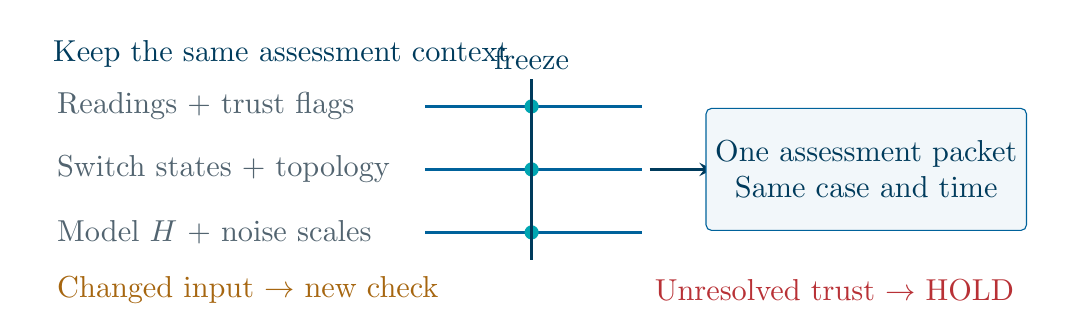
\begin{tikzpicture}[x=1cm,y=1cm,font=\fontsize{11}{13}\selectfont,>=stealth]
\definecolor{IEEEBlue}{HTML}{00629B}
\definecolor{Cyan}{HTML}{00A6B2}
\definecolor{Navy}{HTML}{003B5C}
\definecolor{Slate}{HTML}{526470}
\definecolor{CaseRed}{HTML}{B83136}
\definecolor{Amber}{HTML}{A66610}
\path[use as bounding box] (0,0) rectangle (13,3.5);
\node[anchor=west,text=Navy] at (.2,3.17) {Keep the same assessment context};
\foreach \y/\label in {2.5/{Readings + trust flags},1.7/{Switch states + topology},.9/{Model $H$ + noise scales}} {
  \node[anchor=west,text=Slate] at (.25,\y) {\label};
  \draw[IEEEBlue,line width=1.2pt] (5.05,\y)--(7.8,\y);
  \fill[Cyan] (6.4,\y) circle (.09);
}
\draw[Navy,line width=1.3pt] (6.4,.55)--(6.4,2.85);
\node[anchor=south,text=Navy] at (6.4,2.85) {freeze};
\draw[->,Navy,line width=1.1pt] (7.9,1.7)--(8.7,1.7);
\node[draw=IEEEBlue,rounded corners=2pt,fill=IEEEBlue!5,text=Navy,align=center,minimum width=3.6cm,minimum height=1.55cm] at (10.65,1.7) {One assessment packet\\Same case and time};
\node[anchor=west,text=Amber] at (.25,.17) {Changed input $\rightarrow$ new check};
\node[anchor=east,text=CaseRed] at (12.65,.17) {Unresolved trust $\rightarrow$ HOLD};
\end{tikzpicture}%
